\documentclass[a4paper,12pt]{report}

\usepackage{alltt, fancyvrb, url}
\usepackage{graphicx}
\usepackage{subfigure}
\usepackage{array}
\usepackage{wrapfig}
\usepackage{algorithmic}
\usepackage[utf8]{inputenc}
\usepackage{fontenc}
\usepackage{amsmath,stmaryrd,mathtools,algorithm}
\usepackage{amssymb}
\usepackage{float}
\usepackage{hyperref}

\begin{document}

    
	\title{Elaborato per il corso di Basi di dati}
	\author{Davide Carità - 0000873616}
	\date{}
	
    \maketitle
	\tableofcontents*
	\newpage


	\addcontentsline{toc}{chapter}{Analisi dei requisiti} 
	\chapter*{Analisi dei requisiti}
    Si vuole realizzare una base di dati che supporti le funzionalità di 
    un'applicazione di compravendita di immobili nonché il monitoraggio del 
    welfare delle principali città europee. Uno dei servizi sarà quello di 
    filtrare le città in base alle proprie esigenze: si potrà vedere ad 
    esempio quale città ha ottenuto i migliori punteggi a livello europeo 
    in tema di qualità dell'aria, costo della vita o efficienza sanitaria. 
    Una volta trovata la propria città ideale, verranno visualizzati vari 
    annunci immobiliari suddivisi per zone della città. All'interno 
    dell'annuncio, verranno mostrati i dettagli relativi all'immobile: 
    metratura, numero stanze, prezzo, etc\dots
    Inoltre, il servizio fornirà la funzionalità di avviare una conversazione tra 
    acquirente e venditore, offrendo loro la possibilità di scambiarsi
    informazioni in modo rapido.

    Sarà offerta ai giudici d'esecuzione l'opportunità di creare un utente 
    che avrà il privilegio di gestire aste immobiliari

    	\addcontentsline{toc}{section}{Requisiti in linguaggio naturale} 
        \section*{Requisiti in linguaggio naturale}
    	






    	\addcontentsline{toc}{section}{Estrazione dei concetti principali} 
    	\section*{Estrazione dei concetti principali}
            A seguito della lettura e comprensione dei requisiti richiesti dal cliente, si procede sviluppando un testo che
            ne riassuma tutti i concetti e in particolare ne estragga quelli principali, risultando essere in questo modo
            meglio fruibile per la realizzazione della base di dati.
            
            \begin{center}
                 \begin{tabular}{|c c c|} 
                     \hline
                     Termine & Breve descrizione & Sinonimi \\ [0.5ex] 
                     \hline
                \end{tabular}
            \end{center}
            
            Di seguito le azioni che sono richieste:
            
            \begin{enumerate}
              \item a
              \item b
              \item c
              \item d
              
            \end{enumerate}


	\addcontentsline{toc}{chapter}{Progettazione concettuale}
	\chapter*{Progettazione concettuale}
        La progettazzione concettuale derivata dall'analisi dei concetti principali del dominio
        è stata incrementale in termini di complessità. Di seguito passeremo quindi in rassegna
        gli stadi dello schema cronologicamente ordinati, illustrando le motivazioni che hanno 
        portato ad effettuare i vari raffinamenti.

    	\addcontentsline{toc}{section}{Schema scheletro} 
    	\section*{Schema scheletro}
        \begin{figure}
            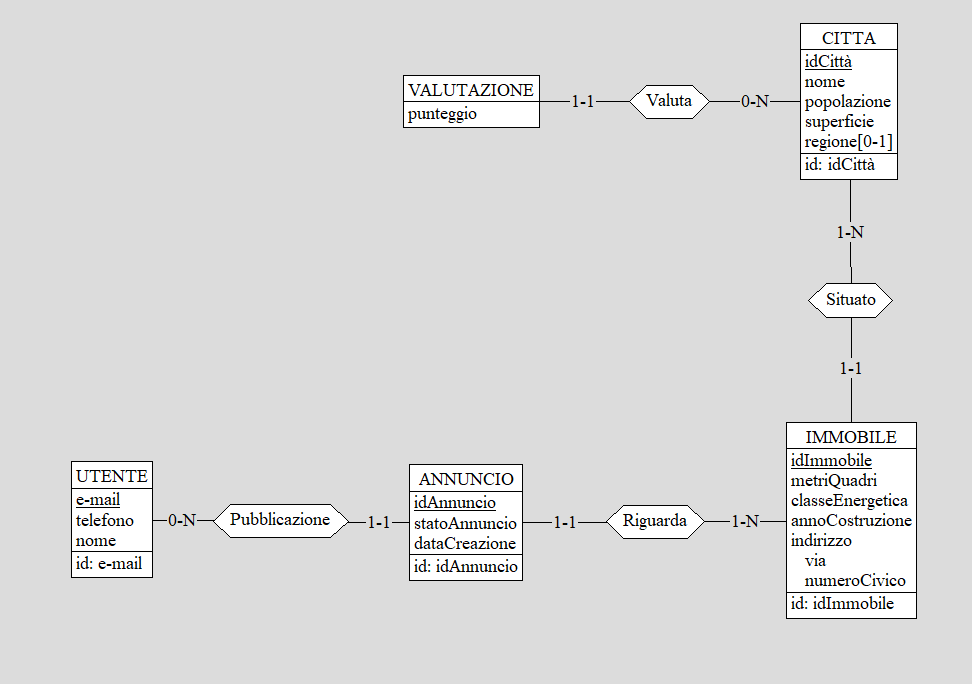
\includegraphics[width=\linewidth]{./images/first.png}
            \caption{La prima versione dello schema concettuale}
        \end{figure}
        
        	
        \addcontentsline{toc}{section}{Schema finale} 
    	\section*{Schema finale}
        	asdasd
        	


        	
    \addcontentsline{toc}{chapter}{Progettazione logica}
	\chapter*{Progettazione logica}
    	\addcontentsline{toc}{section}{Stima del volume dei dati} 
    	\section*{Stima del volume dei dati}
        	asdasd
         	
        \addcontentsline{toc}{section}{Descrizione delle operazioni principali e stima della loro frequenza} 
    	\section*{Descrizione delle operazioni principali e stima della loro frequenza}
        	asdasd
        	
        \addcontentsline{toc}{section}{Schemi di navigazione e tabelle degli accessi} 
    	\section*{Schemi di navigazione e tabelle degli accessi}
        	asdasd
        	
        \addcontentsline{toc}{section}{Analisi delle ridondanze} 
    	\section*{Analisi delle ridondanze}
        	asdasd
        	
        \addcontentsline{toc}{section}{Traduzione di entità e associazioni in relazioni} 
    	\section*{Traduzione di entità e associazioni in relazioni}
        	asdasd
        	
        \addcontentsline{toc}{section}{Schema relazionale finale} 
    	\section*{Schema relazionale finale}
        	asdasd
        	
        \addcontentsline{toc}{section}{Descrizione dell'architettura dell'applicazione realizzata} 
    	\section*{Descrizione dell'architettura dell'applicazione realizzata}
        	asdasd
        	

    \addcontentsline{toc}{chapter}{Progettazione dell'applicazione}
	\chapter*{Progettazione dell'applicazione}
	
    	\addcontentsline{toc}{section}{Traduzione delle operazioni in query SQL} 
    	\section*{Traduzione delle operazioni in query SQL}
    	    asdasd
 
\end{document}